\documentclass[a4paper,11pt]{book}
\usepackage[english]{babel}  
\usepackage[T1]{fontenc} 
\usepackage{helvet} % équivalent Arial

% R real
\usepackage{amsmath}
\usepackage{amssymb}
\newcommand{\R}{\mathbb{R}}

% L Laplace
\usepackage{mathrsfs}

% surlignage
\usepackage{soul}
\sethlcolor{yellow}

\usepackage[usenames]{xcolor}
\definecolor{darkpowderblue}{rgb}{0.0, 0.2, 0.6}
\definecolor{anti-flashwhite}{rgb}{0.95, 0.95, 0.96}
\definecolor{fireenginered}{rgb}{0.81, 0.09, 0.13}
\definecolor{ece}{RGB}{0, 122, 123}
\usepackage[colorlinks=true,linkcolor=black,urlcolor=darkpowderblue,citecolor=darkpowderblue]{hyperref}

\usepackage{listings} % needed for the inclusion of source code
\definecolor{codegreen}{rgb}{0,0.6,0}
\definecolor{codegray}{rgb}{0.5,0.5,0.5}
\definecolor{codepurple}{rgb}{0.58,0,0.82}
\definecolor{backcolour}{rgb}{0.95,0.95,0.92}
\definecolor{ao(english)}{rgb}{0.0, 0.5, 0.0}

\lstdefinestyle{mystyle}{
	backgroundcolor=\color{backcolour},   
	commentstyle=\color{ao(english)},
	keywordstyle=\color{blue},
	numberstyle=\tiny\color{codegray},
	stringstyle=\color{codepurple},
	basicstyle=\footnotesize,
	breakatwhitespace=false,         
	breaklines=true,                 
	captionpos=b,                    
	keepspaces=true,                 
	numbers=left,                    
	numbersep=5pt,                  
	showspaces=false,                
	showstringspaces=false,
	showtabs=false,                  
	tabsize=2
}

\lstdefinelanguage
[x64]{Assembler}     % add a "x64" dialect of Assembler
[x86masm]{Assembler} % based on the "x86masm" dialect
% with these extra keywords:
{morekeywords={CDQE,CQO,CMPSQ,CMPXCHG16B,JRCXZ,LODSQ,MOVSXD, %
		POPFQ,PUSHFQ,SCASQ,STOSQ,IRETQ,RDTSCP,SWAPGS, %
		rax,rdx,rcx,rbx,rsi,rdi,rsp,rbp, %
		r8,r8d,r8w,r8b,r9,r9d,r9w,r9b, %
		r10,r10d,r10w,r10b,r11,r11d,r11w,r11b, %
		r12,r12d,r12w,r12b,r13,r13d,r13w,r13b, %
		r14,r14d,r14w,r14b,r15,r15d,r15w,r15b,bcf,goto,btfsc,btfss,clrf,decfsz,return,incf}} % etc.
\lstset{style=mystyle}
\lstset{language=[x64]Assembler}
\setcounter{chapter}{-1} %starts @Chapter0


% exos sur deux colonnes
%\usepackage[font=it]{caption}% http://ctan.org/pkg/caption
%\usepackage{multicol,lipsum,graphicx,float}
%\usepackage{listings}
%\usepackage{multicol}
%\usepackage{pdflscape}

\definecolor{darkpowderblue}{rgb}{0.0, 0.2, 0.6}
\definecolor{denim}{rgb}{0.08, 0.38, 0.74}
\definecolor{gamboge}{rgb}{0.89, 0.61, 0.06}
\usepackage[pagestyles]{titlesec}
\titleformat{\section}
{\normalfont\fontsize{18}{12}\bfseries\color{ece}}{\thesection}{1em}{}
\titleformat{\subsection}
{\normalfont\fontsize{16}{12}\bfseries\color{ece}}{\thesubsection}{1em}{}
\titleformat{\subsubsection}{\normalfont\fontsize{15}{15}\bfseries\color{gamboge}}{\thesubsection}{1em}{}


%symboles
\usepackage{bclogo}


%F10 key
\usepackage{tikz}
\usetikzlibrary{shadows}
\newcommand*\keystroke[1]{%
	\tikz[baseline=(key.base)]
	\node[%
	draw,
	fill=white,
	drop shadow={shadow xshift=0.25ex,shadow yshift=-0.25ex,fill=black,opacity=0.75},
	rectangle,
	rounded corners=2pt,
	inner sep=1pt,
	line width=0.5pt,
	font=\scriptsize\sffamily
	](key) {#1\strut}
	;
}


% code
\usepackage{verbatim}

\newcommand{\HRule}[1]{\rule{\linewidth}{#1}}

%subfigure
\usepackage{graphicx,subcaption}
\usepackage{ragged2e}

% next year command

\newcommand\NextYear{%
	\advance\year by 1 \the\year\advance\year by -1}


% "Figure" en gras
\usepackage[labelfont=bf]{caption}

%tableaux horizontaux
\usepackage{booktabs}

%auteurs page de garde
\usepackage[affil-it]{authblk}
\makeatletter
\def\@maketitle{%
	\newpage
	\null
	\vskip 2em%
	\begin{center}%
		\let \footnote \thanks
		{\Large\bfseries \@title \par}%
		\vskip 1.5em%
		{\normalsize
			\lineskip .5em%
			\begin{tabular}[t]{c}%
				\@author
			\end{tabular}\par}%
		\vskip 1em%
		{\normalsize \@date}%
	\end{center}%
	\par
	\vskip 1.5em}
\makeatother

%numérotation parties / chapitres (reset counter)
\usepackage{hyperref}
%\usepackage{chngcntr}


% angstrom
\usepackage{siunitx}

% L lagrangien
\usepackage{ amssymb }

%caption dans minipage
\usepackage{caption}


% graphes
\usepackage{tikz}
\usepackage{xlop}
\newcommand*{\prettyprint}[1]{\opcopy{#1}{a}\opunzero{a}\opprint{a}}
\usepackage{pgfplots}



%signe euro
\usepackage{eurosym}

%ajout pdf
\usepackage[final]{pdfpages}

% sommaire
\usepackage[tight]{shorttoc}

% adresse mail
\usepackage{hyperref}
\newcommand{\email}[1]{\href{mailto:#1}{\nolinkurl{#1}}}
\urlstyle{sf}

% images
\usepackage{graphicx}

% maths
\usepackage{amssymb}
\usepackage{amsmath}
\usepackage{esint}

% part sans nvlle page
\usepackage{titlesec}
\titleclass{\part}{top}
\titleformat{\part}[display]
{\normalfont\huge\bfseries}{\centering\partname\ \thepart}{20pt}{\Huge\centering}
\titlespacing*{\part}{0pt}{50pt}{40pt}


% sous-subsection
\setcounter{secnumdepth}{4}
\setcounter{tocdepth}{4}
\makeatletter
\newcounter {subsubsubsection}[subsubsection]
\renewcommand\thesubsubsubsection{\thesubsubsection .\@alph\c@subsubsubsection}
\newcommand\subsubsubsection{\@startsection{subsubsubsection}{4}{\z@}%
	{-3.25ex\@plus -1ex \@minus -.2ex}%
	{1.5ex \@plus .2ex}%
	{\normalfont\normalsize\bfseries}}
\renewcommand\paragraph{\@startsection{paragraph}{5}{\z@}%
	{3.25ex \@plus1ex \@minus.2ex}%
	{-1em}%
	{\normalfont\normalsize\bfseries}}
\renewcommand\subparagraph{\@startsection{subparagraph}{6}{\parindent}%
	{3.25ex \@plus1ex \@minus .2ex}%
	{-1em}%
	{\normalfont\normalsize\bfseries}}
\newcommand*\l@subsubsubsection{\@dottedtocline{4}{10.0em}{4.1em}}
\renewcommand*\l@paragraph{\@dottedtocline{5}{10em}{5em}}
\renewcommand*\l@subparagraph{\@dottedtocline{6}{12em}{6em}}
\newcommand*{\subsubsubsectionmark}[1]{}
\makeatother
\usepackage{hyperref}
\makeatletter
\def\toclevel@subsubsubsection{4}
\def\toclevel@paragraph{5}
\def\toclevel@subparagraph{6}
\makeatother

% numérotation sous sous section en lettre
\renewcommand{\thesubsubsection}{\alph{subsubsection}}


%marges
\usepackage[margin=2cm]{geometry}

% texte en couleur
\usepackage{color}


% en-tête de page
\usepackage{fancyhdr}
\usepackage{lastpage}
\lhead{	
\includegraphics[width=0.15\linewidth]{ece.png}}
\cfoot{\thepage}
\pagestyle{fancy}

%fraction spéciale
\newcommand*\rfrac[2]{{}^{#1}\!/_{#2}}

%lignes horizontale tableau épais
\usepackage{makecell}

% images
\usepackage{graphicx}

% maths
\usepackage{amssymb}
\usepackage{amsmath}

%\fancyfoot[L]{M. Schneider}
\fancyfoot[R]{}
\fancyfoot[L]{ING{3}}


%fancy chapter presentation
\usepackage[Lenny]{fncychap}
%\ChNameVar{\Large \textbf{Laboratory Session}}

%\ChNumVar{\fontsize{90}{92}\bfseries}
%\ChTitleVar{\Huge\textbf{\thechapter}}
\usepackage{ifthen}
\makeatletter
\renewcommand{\@chapapp}{TP n$^{\text{o}}$}
\makeatother
\ChNameVar{\fontsize{20}{22}\usefont{OT1}{phv}{m}{n}\selectfont}
\ChNumVar{\fontsize{60}{62}\usefont{OT1}{ptm}{m}{n}\selectfont}
\ChTitleVar{\Huge\bfseries\rm}
\ChRuleWidth{1pt}

\renewcommand{\headrulewidth}{0pt}


%symboles drapeaux
\usepackage{bclogo}


\begin{document}
	
	\begin{titlepage}
	\title{\vspace{-5em}
		\begin{figure}[htb]
			\begin{minipage}[t]{.45\textwidth}
				\centering
				
\includegraphics[width=\textwidth]{ece.png}
			\end{minipage}
			\hfill
			\begin{minipage}[t]{.45\textwidth}
				\centering
				\flushright\vspace{-12mm}\Large{\textbf{ING{3}}\\ Groupe {5}}
			\end{minipage}  
		\end{figure}
		\normalsize \textsc{} \\ [1.2cm]
		\HRule{1.5pt} \\ [0.5cm]
		\LARGE \textbf{\Large{RAPPORT DE PROJET}\\ \vspace{5mm}
			\Huge{\textcolor{ece}{PROJET : {Reconnaissance vocale}}}}
		\HRule{1.5pt} \\ 
		\normalsize  \vspace{1cm}
		\fcolorbox{white}{anti-flashwhite}{\begin{minipage}{16cm}\vspace{4cm}\textbf{RÉSUMÉ} – Quel est le contexte et la problématique du projet ? Quels sont les objectifs techniques ? Dans quel contexte faites-vous ce projet ? [maximum 20 lignes]	\vspace{4cm}\end{minipage}}}
	\date{Mathis ESMILLER, Clément LAMBERT, Thomas LOPEZ\\ Nous attestons que ce travail est original, qu’il est le fruit d’un travail commun au binôme et qu’il a été rédigé de manière autonome. \\ \textbf{{Paris, le 15/05/2022}}}
	
	\author{}
\end{titlepage}
	

	
	
	\maketitle
\section*{Table des matières}
\begin{tabbing}
\textbf{{I. Objectifs ............................................................................................................. p. XX}}\\
\textbf{{II. Glossaire ........................................................................................................... p. XX}}\\
A. Termes ................................................................................................................................... p. XX\\
B. Acronymes ............................................................................................................................. p. XX\\
\textbf{{III. L'équipe ......................................................................................................... p. XX}}\\
A. Présentation de l'équipe ...................................................................................................... p. XX\\
B. Organisation de l'équipe ........................................................................................................ p. XX\\
C. Diagramme de GANTT ......................................................................................................... p. XX\\
\textbf{{IV. Contexte et problématique ................................................................................ p. XX}} \\
A. Contexte ................................................................................................................................ p. XX\\
B. Problématique ....................................................................................................................... p. XX\\
C. Spécifications techniques ....................................................................................................... p. XX\\
\textbf{{V. Conception ...................................................................................................... p. XX}}\\
A. Architecture fonctionnelle ...................................................................................................... p. XX\\
B. Architecture matérielle ........................................................................................................... p. XX\\
C. Architecture logicielle ............................................................................................................ p. XX\\
\textbf{{VI. Développement ................................................................................................. p. XX}}\\
A. Module 1 ................................................................................................................................ p. XX\\
B. Module 2 ................................................................................................................................ p. XX\\
C. Module 3 ................................................................................................................................ p. XX\\
\textbf{{VII. Tests et validation ............................................................................................ p. XX}}\\
A. Module 1 ................................................................................................................................ p. XX\\
B. Module 2 ................................................................................................................................. p. XX\\
C. Module 3 ................................................................................................................................. p. XX\\
\textbf{{VIII. Bilan ............................................................................................................... p. XX}}\\
A. État d'avancement .................................................................................................................. p. XX\\
B. Pertinence de la solution technique ........................................................................................ p. XX\\
C. Bilan sur le travail d'équipe .................................................................................................... p. XX\\
\textbf{{IX. Sources .......................................................................................................... p. XX}}\\
\textbf{{X. Annexes ............................................................................................................ p. XX}}\\
\end{tabbing}








\newpage
\section*{I. Objectifs}
L'objectif de ce rapport est d'expliquer les différents objetifs de ce projet ainsi que les différentes étapes par lesquelles nous sommes passés pour y arriver. Nous abordons également le déroulement du projet de reconnaissance vocale d'un point de vu organisationnel et technique.\\ \\
\unindent {La reconnaissance vocale consiste en l'analyse de la voix humaine, afin de la transformer en données utilisables pour réaliser des actions voulues. Tout passe par la voix, qui est identifiée puis captée en fréquences sonores. Vient ensuite l'analyse de ces fréquences sonores pour arriver à des données exploitables dans le cadre de notre projet. \\ \\

Le but de ce projet est de créer un circuit électronique qui réceptionne un signal, le filtre afin de reconnaître la fréquence des signaux reçus, faire sa transformée de Fourier afin d'en déterminer les harmoniques nous permettant de reconnaître si le signal capté vient d'un utilisateur A, B ou C et d'agir en conséquence.}\\ \\

\unindent {Le lecteur trouvera dans ce rapport différentes ressources utilisées et les documents produit nécessaires au bon déroulement du projet, des explications théoriques ainsi que des exemples imagés de nos réalisations pratiques.}\\

\newpage
\section*{II. Glossaire}
\subsection*{A. Termes}
Renseigner ici sous forme de tableau les principaux termes techniques et leurs définitions.

\subsection*{B. Acronymes}
Renseigner ici sous forme de tableau les principaux acronymes, leurs signification et leurs explication.

\newpage
\section*{III. L'équipe}
\subsection*{A. Présentation de l'équipe}
Notre équipe est composé de trois élèves:\\ \\

\textbf{Mathis ESMILLER}.\\
Spécialiste en électronique, Mathis sera l'année prochaine en majeur Système Embarquée, c'est pour cette raison qu'il a été le plus à même de remplir le poste de chef de projet en guidant les deux autres membres du projet. À l'aise avec les montages électroniques sur breadboard et dans la théorie, la reconnaissance vocale est le type de projet qui lui permet de s'épanouir au sein de l'ECE. A déjà collaboré avec Thomas lors du projet en JAVA de début de semestre. \\

\textbf{Clément LAMBERT}.\\
Futur OCRES, Clément a su participer activement et efficacement à ce projet d'électronique grâce à sa capacité d'adaptation et ses connaissances en électronique. À l'aise avec l'électronique théorique, il lui tenait à cœur d'aider au bon déroulement du projet. \\

\textbf{Thomas LOPEZ}.\\
Futur OCRES également, Thomas a comme qualités principales l'informatique (Arduino), un esprit de synthèse développé et la gestion de projet. Il a pour habitude de mener l'ensemble des projets auxquels il participe à bien. A déjà collaboré avec Mathis sur le projet d'informatique en JAVA. \\ 

\subsection*{B. Organisation de l'équipe}
Mathis, chef de projet, le plus à l'aise en électronique du groupe, il a principalement travaillé sur le montage électronique du projet, une partie de l'Arduino ainsi que le modèle de l'IA permettant de détecter les commandes oralement évoquées. \\

Clément, compétent en électronique théorique, a su faire preuve de rigueur dans ses démonstrations pour prouver de façon théorique le montage dont nous avons besoin pour réaliser la reconnaissance vocale à partir de l'Arduino donnée ainsi que les valeurs des composants choisies. Il a été un vecteur de communication entre Mathis et Thomas ainsi qu'une grande aide dans la conception du modèle de l'IA grâce à son expérience dans la matière acquerit lors de son semestre à l'international. \\


Thomas, en ses qualités de développeur, a travaillé principalement sur le code Arduino à partir de la bibliothéque Arduino sur la FFT ainsi que sur le rapport en collaboration avec Clément. Il a également apporté son expérience acquise en dehors des cours en gestion de projet pour organiser l'avancement de ce projet d'électronique. \\

\subsection*{C. Diagramme de Gantt}
Comment est utilisé le temps alloué au projet ? 

\includegraphics[width=\textwidth]{Diagramme de gantt.png}

\newpage
\section*{IV. Contexte et problématique}
\subsection*{A. Contexte}
Considéré aujourd'hui comme gadgets high-tech, les assistants à reconnaissance comme Siri (Apple) ou Alexa (Amazon) sont vendus à plus de 200 millions d'exemplaires à travers le monde. Un nombre important lié au phénomène de full connectivité amenée par la digitalisation de notre monde, les utilisateurs ne veulent plus utiliser de télécommandes pour commander les appareils électroniques de leur domicile. \\ \\
Économiquement, on peut donc dire que la reconnaissance vocale est applicable au moins à ce type d'applications de full connectivité, croissantes sur le marché. Relativement simple à faire, la marge réalisée sur la vente est presque entièrement réalisée par la plus-value technologique apportée par la conception électronique et informatique du produit. \\ 
De plus, les GAFA, leaders de ce type de solutions réalisent de nombreux revenus grâce à l'ensemble des données récupérées lors de l'utilisation de leur produit utilisant la reconnaissance vocale. \\ \\

Socialement, cette dernière proposition a un fort impact sur les données des utilisateurs censée être privées mais leur besoin de connectivité à domicile a pris le dessus malgrès les scandales provoqués, ce qui traduit un potentiel de marché gigantesque dû à un atout technologique répondant à un besoin croissant. D'un point de vue social, ce type de produit permet à de nombreuses personnes seules de se sentir accompagnées bien que le compagnon ne soit pas tangible. On peut également souligné l'impact social qu'a eu ce type de produits sur une population passant de moins en moins de temps dehors, lors des confinements dûs à la pandémie mondiale les ventes d'assistants à reconnaissance vocale a augmenté. \\ 
Il est également soulignable que ce type de solutions aident fortement les personnes agées ne sachant pas utiliser la technologie d'aujourd'hui ainsi que les handicapés physiques ppouvant contrôler de nombreux paramètres de leur domicile sans bouger.\\ \\

Enfin, sur un plan écologique, le constat est moins bon, comme dans la plupart des milieux de la tech de nombreux composants ne sont pas recyclables et la production délocalisée dans les pays asiatiques fait que l'acquisition d'un produit utilisant la reconnaissance vocale aura coûté de nombreux kilomètres de trajets. D'un point de vue beaucoup plus centré sur notre projet à l'ECE Paris, du fait de nombreux tests, composants déffectueux ainsi que conseils ou ressources envoyée non fonctionnelles, nous avons cramé des composants, choses évitables et regrettables.\\ \\ \\ \\ \\

\noindent Un point d'histoire pour commencer, les travaux sur la reconnaissance de la parole datent du début du xxe siècle. Le premier système pouvant être considéré comme faisant de la reconnaissance de la parole date de 1952. Ce système avait pour objectif de reconnaître des chiffres isolés à l'aide de la voix uniquement. \\ 
Il s'en est suivi un développement exponentielle de la technologie, en passant par une reconnaissance des mots isolés, les premiers produits commerciaux de reconnaissances de mots, commercialisation d'un système de reconnaissance à microprocesseurs sur une carte de circuits imprimés, les premières commandes vocales à bord d'avion de chasse (commande française) avant de s'orienter vers des téléphones avec traduiction automatiques ainsi que comme évoqué précédemment les assistants à reconnaissance vocale à domicile et l'IA associé à cette reconnaissance vocale, Alexa ou Siri. \\ \\
Avec une technologie évoluant aussi vite, il est important de pouvoir se projet sur son utilisation futures et ses limites. \\ \\
Avec la récupération des données utilisateurs par les GAFA, nous sommes obligé de parler des potentielles dérives de ces technologies pouvant être utilisé à des fins de suivi de la population dans les lieux publics pour le pire scènario. Dans un scènario plus positif on peut penser à une digitalisation de l'ensemble des commandes grâce à la reconnaissance vocale, ce qui permettrait d'éviter les contacts avec des bornes publiques et donc limiter les échanges de bactéries / maladies, il est également possible d'aborder la démocratisation de la sécurité basée sur la détection de la voix de l'utilisateur, difficilement reproductible. \\ \\

\subsection*{B. Problématique}
Notre projet répond à la problèmatique suivante: \\ \textbf{Comment utiliser un appareil électronique à l'aide de la voix ou des sons produits uniquement ?} \\ \\

\subsection*{C. Spécifications techniques}
Les spécifications techniques du projet ne sont pas nombreuses mais il est nécessaire de les lister: \\ \\
\begin{itemize}
        \item \textbf{Utilisation d'une Arduino Nano.}
        \item \textbf{Utilisation d'un micro fourni par l'école.}
        \item \textbf{Passez par la transformée de Fourier à partir de la bibliothèque Arduino FFT.} 
\end{itemize}
\vspace{2mm}

\newpage
\section*{V. Conception}
\subsection*{A. Architecture fonctionnelle}
L'architecture fonctionnelle du projet, regroupant toutes les fonctionnalité réalisées s'organise comme suit: 
\begin{itemize}
        \item Capter le signal sonore émit grâce au circuit électronique équipe d'un micro
\indent \item Filtrer le signal
\indent \item Récupérer le signal et afficher sur l'écran LED intégré au circuit 
\indent \item Afficher la courbe de ce signal sur le traceur série dans l'application Arduino 
\indent \item Transformer ce signal temporel en fréquentiel grâce à l'analyse de Fourier 
\indent \item Détecter avec les premières harmoniques l'empreinte fréquentielle d'une voix
\indent \item Corréler notre IA pour reconnaître la commande vocale saisie par l'utilisateur, 1,2,3 ou clap 
\indent \item Actionner des fonctionnalités correspondantes selon ces harmoniques 
\indent \item Effectuer ces actions et les afficher sur l'écran LED du circuit 
\end{itemize}

\vspace{3mm}
\subsection*{B. Architecture matérielle}
Pour ce projet, nous avons réalisé des montages par nous même sans succès avant de nous inspirer d'un montage proposé par M.Derraz pour faire le notre. Ce dernier se trouve ci-dessous:

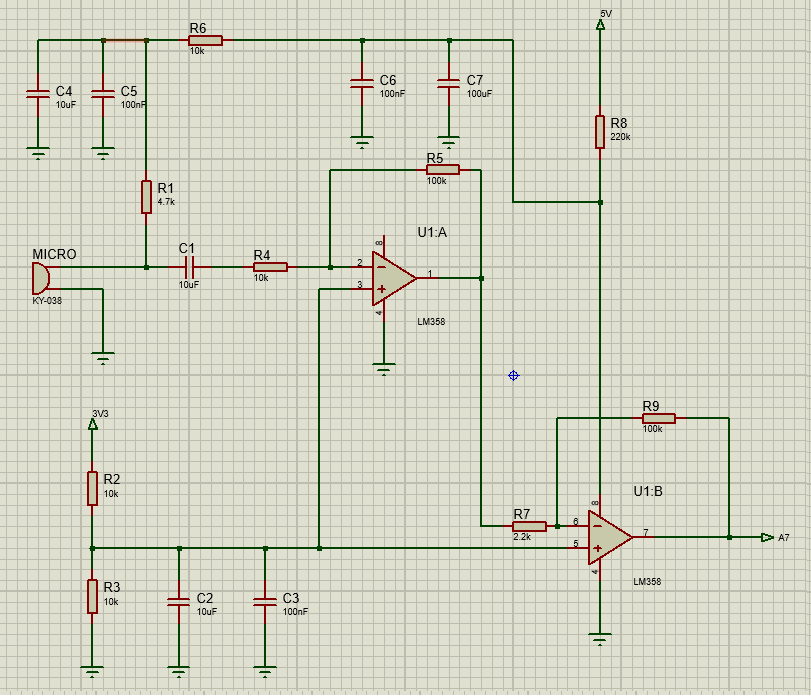
\includegraphics[width=\textwidth]{template_PRJ_TEX_FR/montageprojet.png} \\
\begin{center} \underline{\textbf{Schéma de notre montage sur Proteus}} 
\end{center}

\subsection*{C. Architecture logicielle}
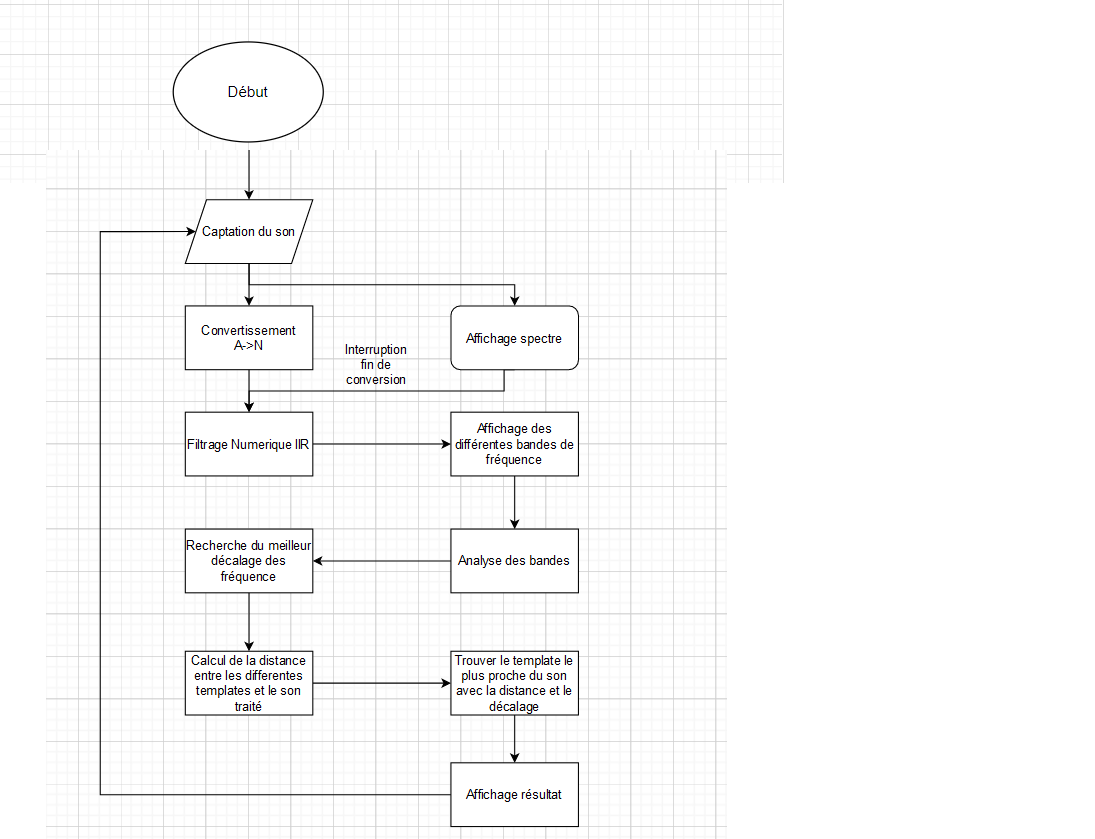
\includegraphics[width=\textwidth]{template_PRJ_TEX_FR/algorigramme.png}
\begin{center} \underline{\textbf{Algorigramme du projet}} 
\end{center}
Voici ci-dessus un algorigramme représentant le fonctionnement du code de notre programme et les différentes étapes pour la réalisation des fonctions demandées.

\newpage
\section*{VI. Développement}

\subsection*{A. Module 1: Amplification du signal }
L'amplification du signal est un élément clé de notre projet puisque le microphone que nous utilisons, le capteur de son KY-038, est assez peu sensible et par conséquent, les signaux reçus doivent être amplifiés.\\ 
Le micro comporte 2 LEDs: une qui est allumée quand le capteur est alimenté, et la deuxième qui est normalement allumée uniquement lorsqu'un son est détecté. 
Nous avons donc du ajuster le potentiomètre de notre micro en premier lieu afin que cette dernière ne soit allumée qu'en présence de son. Pour cela il nous a fallu le tourner dans le sens des aiguilles d'une montre jusqu'à ce que la valeur analogique lue atteigne environ 512 vu que l'ADC de 10 bits peut comporter 2 à la puissance 10 valeurs, soit 1024 valeurs. \\  
La pleine échelle d'un convertisseur analogique-numérique est divisée en autant de plages d’égale dimension qu’il y a d’états possibles de la sortie numérique. Chaque plage est associée à un code numérique représentant la tension analogique d’entrée. Ainsi, grâce à l'amplification du signal d'entrée, nous obtenons un signal en pleine échelle entre 0V et 5V. Notre projet présente également un filtre anti repliement afin d'éviter tout recouvrement de spectre lors de la transformation de Fourier. La fréquence maximale captée par notre micro est de 5kHz, nous avons donc du respecter la condition de Shannon, à savoir Fe > 2*Fmax aet avons donc pris une fréquence d'échantillonnage de 15kHz.

\subsection*{B. Module 2: Afficher en temps réel le spectre en amplitude}
Pour afficher le spectre du signal, nous nous sommes servi du TP2 réalisé précédemment durant le semestre. Celui-ci utilise les fonctions de FFT de la librairie du même nom pour transformer notre signal dans le domaine fréquentiel puis le visualiser à l'aide de l'écran OLED de notre circuit. \\ 
Grâce à la fréquence d'échantillonnage élevée que nous avons choisie et à la vitesse de lecture et de conversion du signal, nous pouvons observer clairement le spectre de notre signal en temps réel avec une amplitude précise. Nous avons également développé une fonction qui permet d'afficher les décibels mesurés et d'afficher la valeur également sur notre écran OLED.

\subsection*{C. Module 3: Allumer / éteindre toutes les LEDs lorsque l’on claque des mains }

Ce module est en quelque sorte la base de notre projet puisqu'il représente la première fonctionnalité qui répond directement à la problématique de notre projet à savoir réaliser une action à partir de voix ou de sons générés. \\ 
Pour ce module, nous avons tout d'abord utilisé un filtre qui permet d'éliminer les basses fréquences, de façon à ce que le bruit ambient ne soit pas détecté et donc que le capteur ne se déclenche pas de manière intempestive sans qu'on le veuille. Nous avons établi qu'un "clap" se caractérise par un bruit fort et très court qui sera plus facilement mis en évidence par l'amplificateur opérationnel. Ainsi lorsqu'un tel bruit sera détecté, les 3 LEDs de notre circuit vont s'allumer si elles étaient éteintes et s'éteindre si elles étaient allumées. \\ 

\subsection*{D. Module 4: Reconnaitre « un », « deux » et « trois » pour allumer / éteindre la 1ère, 2nde }

C'est à partir du module précédent que nous avons effectué celui-ci. En effet, sur le même principe nous avons fait en sorte que lorsque l'on dit "un" et que ce son est capté par notre micro, alors la LED numéro 1 s'allume ou s'éteint en fonction de l'état dans lequel elle était, de même pour les autres LEDs. Cela est possible grâce au machine learning que nous avons effectué: nous avons appris à notre système quelles actions il doit réaliser en fonction de ce qu'il capte. A force d'entrainement, la précision devient de plus en plus grande et notre système reconnait de mieux en mieux les informations qu'on lui transmet.


\newpage
\section*{VII. Tests et validation}

\vspace{2mm}
\noindent Il est question ici de montrer les performances techniques du système et de valider le développement module par module puis au global (intégration) en accord avec la partie IV.

\vspace{2mm}

\noindent \textbf{Test concernant l'entrainement de notre modèle d'IA} : 
\begin{itemize}
	\item Nous avons réalisé à un modèle d'IA en Arduino afin d'améliorer la précision des signaux captés et mieux reconnaître les lettres/chiffres/claps captés;
	\item On est censé obtenir une suite de courbe qui se lisse au fur et à mesure des tests grâce au machine learning pour au final avoir une courbe "moyenne" du signal correspondant au mot capté par le micro;
	\item Ce que l’on obtient est visible sur la photo ci-dessous, nous avons entrainé notre modèle pour détecter au mieux les chiffres 1,2,3 et un clap comme demandé dans le brief du projet: \\ \\
	\vspace{2mm}
	\includegraphics[width=\textwidth]{training_IAArduino.png}
	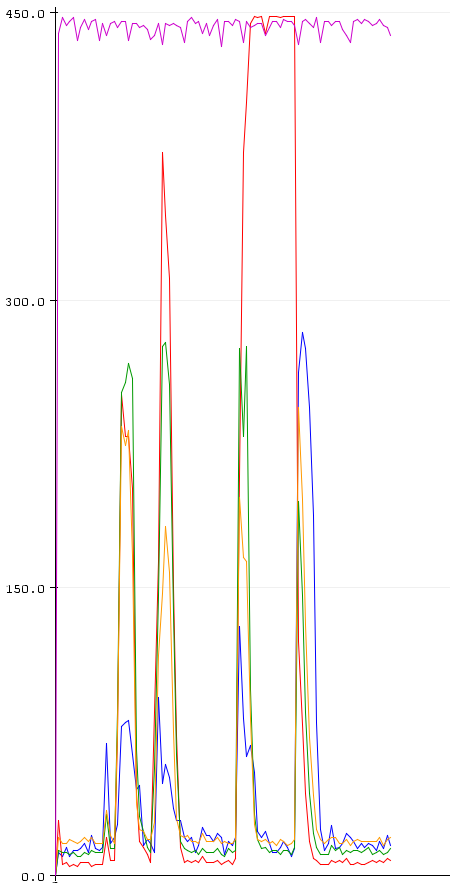
\includegraphics[width=\textwidth]{test_123clap.png} \\ \\  
	\item On voit distinctement sur les photos ci-dessus que cet entrainement de notre IA est totalement fonctionnel et que les tests donne ce que nous voulons, à savoir une meilleure détection des signaux correspondant aux commandes vocales 1,2,3 et le clap.
\end{itemize}

\vspace{3mm}

\subsection*{A. Module 1}
\subsection*{B. Module 2}
\subsection*{C. Module 3}

\newpage
\section*{VIII. Bilan}
\subsection*{A. État d'avancement}
Où en est le projet ? A-t-on atteint les objectifs ?\\
\noindent Quels modules restent à finaliser (ou à perfectionner pour être en accord avec les spécifications techniques) ?

\subsection*{B. Pertinence de la solution technique}
Quelles sont les limites techniques de la solution développée ? \\
\noindent Quelles sont les possibilités d’évolution ou de poursuite ?


\subsection*{C. Bilan sur le travail d'équipe}
Qu’avez-vous appris individuellement ? Quelles compétences vont pouvoir être mises en avant lors de votre prochaine recherche de stage ?
\\
\noindent Comment l’équipe aurait pu mieux s’organiser ? Proposer un plan d’action pour le prochain projet.



\newpage
\section*{IX. Sources}
Documents utilisés et sites internet consultés pour développer le projet.\\
\noindent \textbf{NB} : voir le document « comment rédiger un rapport » sur la page Moodle La Toolbox pour la syntaxe à utiliser pour vos citations.



\newpage
\section*{X. Annexes}
Documents annexes, éventuels codes (\textbf{\textcolor{red}{pas de code dans le rapport}}).











\end{document}
